% This file defines the command for plotting the standard normal PDF and CDF.
% It can be compiled standalone or included in a larger document.

\ifdefined\ispartofbook
\else
  % --- Standalone Compilation Preamble ---
  \documentclass[tikz, border=10pt]{standalone}
  \usepackage{tikz}
  \usetikzlibrary{arrows.meta}
  % No longer need pgfplots, as we are using pre-computed coordinates
  \begin{document}
\fi

% --- THE DIAGRAM COMMAND ---
\newcommand{\normalpdfcdfplot}{%
    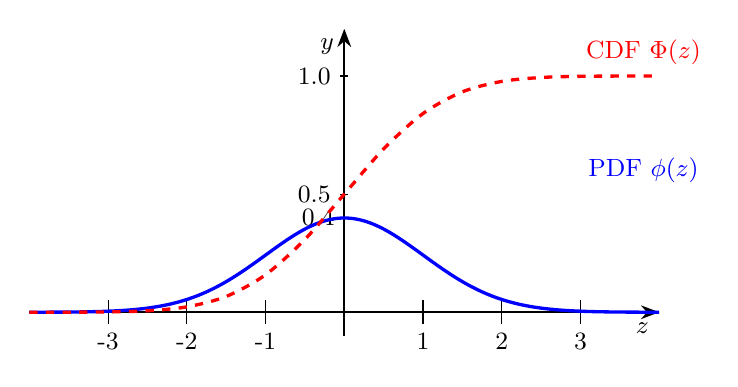
\begin{tikzpicture}[
        x=1cm, y=3cm, % Set vertical unit larger than horizontal to make plot taller
        font=\sffamily,
        every node/.style={font=\small}
    ]
    % Axes
    \draw[-Stealth, thick] (-4,0) -- (4,0) node[below left] {$z$};
    \draw[-Stealth, thick] (0,-0.1) -- (0,1.2) node[below left] {$y$};

    % Axis labels
    \foreach \x in {-3, -2, -1, 1, 2, 3}
        \draw (\x, 0.05) -- (\x, -0.05) node[below] {\x};
    \foreach \y/\ytext in {0.5/{0.5}, 1/{1.0}}
        \draw (0.05, \y) -- (-0.05, \y) node[left] {\ytext};
    \node[left] at (0, 0.4) {0.4}; % For PDF peak

    % PDF plot (bell curve) using the built-in gaussian function
    \draw[blue, very thick, smooth, domain=-4:4, samples=100] plot (\x, {1/sqrt(2*pi)*exp(-(\x*\x)/2)});

    % CDF plot (S-shaped curve) using pre-computed coordinates to avoid 'erf' dependency
    \draw[red, very thick, dashed, smooth] plot coordinates {
        (-4.0, 0.00003) (-3.5, 0.0002) (-3.0, 0.0013) (-2.5, 0.0062) 
        (-2.0, 0.0228) (-1.5, 0.0668) (-1.0, 0.1587) (-0.5, 0.3085) 
        (0.0, 0.5) (0.5, 0.6915) (1.0, 0.8413) (1.5, 0.9332) 
        (2.0, 0.9772) (2.5, 0.9938) (3.0, 0.9987) (3.5, 0.9998) 
        (4.0, 0.99997)
    };
    
    % Legend
    \node[blue, align=right] at (3.8, 0.6) {PDF $\phi(z)$};
    \node[red, align=right] at (3.8, 1.1) {CDF $\Phi(z)$};
    
    \end{tikzpicture}%
}

\ifdefined\ispartofbook
  % This part is intentionally left blank when included in the main book.
  % The \newcommand is defined, and the chapter file is responsible for calling it.
\else
  % This part is for standalone compilation of the image.
  \normalpdfcdfplot
  \end{document}
\fi
